\section{Introduction}
A server room monitoring system panel is an essential component for ensuring the proper functioning of a server room environment. It provides real-time monitoring of key physical and environmental factors such as temperature, humidity, power, and network connectivity. The panel alerts administrators in case of any deviations from the defined thresholds, helping prevent potential data loss, hardware damage, and downtime. Additionally, this system provides historical data and reporting capabilities, allowing administrators to track trends and make informed decisions about capacity planning and infrastructure improvements. With the right server room monitoring system panel in place, organizations can ensure the safety and reliability of their critical IT assets.
\section{Back-end}
Node.js, PostgreSQL, and Prisma can be used together to build a robust and scalable back-end for a server room monitoring panel.
    \subsection{Node js} 
    Node.js is a JavaScript runtime built on Chrome's V8 JavaScript engine, and is a critical component in building a server room monitoring panel's back-end. Node.js allows developers to use JavaScript on the server-side, providing a unified language for both client-side and server-side development. This helps to simplify the development process and increase developer productivity.\\
    In a server room monitoring panel's back-end, Node.js can be used to create APIs or other server-side components that provide data for the monitoring panel. For example, it can be used to create a REST API that retrieves data from a database or other source and returns it in a format that can be consumed by the monitoring panel. Node.js is also well-suited for building fast and scalable applications, making it a good choice for a server room monitoring panel's back-end. Its asynchronous, non-blocking I/O model ensures that the back-end can handle a large number of concurrent requests without becoming slow or unresponsive \cite{nodejs}.
    \subsection{Postgresql}
    PostgreSQL is an open-source relational database management system (RDBMS) and is a critical component in building the back-end for a server room monitoring panel. PostgreSQL is a powerful and reliable database system that can be used to store the data collected by the monitoring panel, such as temperature, humidity, power, and network connectivity. It provides a range of features for managing and querying data, including support for SQL, transactions, and advanced data types.
    The use of a relational database, such as PostgreSQL, is important for a server room monitoring panel because it ensures the data is stored in a structured manner. This makes it easier to retrieve and analyze the data, and also provides a robust solution for managing the data over time, ensuring its reliability and longevity. PostgreSQL also provides security features, such as user authentication and access control, to ensure that the data stored in the database is protected. This is especially important for a server room monitoring panel where sensitive information, such as server uptime, may be stored \cite{postgresql}.
    \subsection{Prisma} 
    Prisma is a modern database toolkit that provides a high-level API for working with databases and is a critical component in building the back-end for a server room monitoring panel. Prisma allows developers to work with databases, such as PostgreSQL, in a type-safe and efficient manner. It provides a set of TypeScript types for the data stored in the database, making it easy to catch bugs and errors at compile time. This helps to ensure the quality and reliability of the data stored in the database.\\
    Prisma also provides a query builder for constructing and executing SQL queries, allowing developers to retrieve the data necessary for the monitoring panel. This makes it easy to retrieve and manipulate the data stored in the database, while also providing the performance and efficiency necessary for a server room monitoring panel's back-end. Prisma also provides a streamlined and modern API for working with databases, making it easier for developers to build robust and scalable back-ends. This can help to reduce development time and increase developer productivity \cite{prisma}.
\section{Front-end}
    \subsection{React}
    React is a JavaScript library for building user interfaces, and is a critical component in building a server room monitoring panel. React allows for the creation of reusable components, making it easier to manage and maintain the codebase as the application grows in complexity. This helps to ensure that the monitoring panel is both scalable and flexible, allowing for new features and functionality to be added as needed.\\
    In a server room monitoring panel, React can be used to create components for displaying real-time data, such as temperature, humidity, power, and network connectivity. This data can be fetched from APIs or other sources and dynamically updated using React's state management. This helps to ensure that the monitoring panel provides an up-to-date and accurate representation of the server room environment at all times. React's hooks and context also make it easy to add alerts and notifications to the monitoring panel, ensuring that administrators are promptly notified of any deviations from the defined thresholds. This helps to prevent potential data loss, hardware damage, and downtime \cite{react}.
    \subsection{Next js}
    Node.js is a JavaScript runtime built on Chrome's V8 JavaScript engine, and is a critical component in building a server room monitoring panel. Node.js allows developers to use JavaScript on the server-side, providing a unified language for both client-side and server-side development. This helps to simplify the development process and increase developer productivity.\\
    In a server room monitoring panel, Node.js can be used to create APIs or other server-side components that provide data for the monitoring panel. For example, it can be used to create a REST API that retrieves data from a database or other source and returns it in a format that can be consumed by the monitoring panel.\\
    Node.js is also well-suited for building fast and scalable applications, making it an appropriate choice for a server room monitoring panel. Its asynchronous, non-blocking I/O model ensures that the monitoring panel can handle a large number of concurrent requests without becoming slow or unresponsive \cite{nextjs}.
    \subsection{Tailwind}
    Tailwind is a utility-first CSS framework, and is a critical component in building a server room monitoring panel. Tailwind provides a set of pre-defined CSS classes for quickly building responsive and customizable designs. This helps to significantly speed up the development process, as developers do not need to write custom CSS for common design elements.\\
    In a server room monitoring panel, Tailwind can be used to style the components created with React. It provides a wide range of classes for controlling layout, typography, colors, and more, making it easy to create a consistent and professional look and feel for the monitoring panel. Tailwind also provides a set of responsive design classes, allowing the monitoring panel to adjust its layout and appearance based on the size of the user's screen. This helps to ensure that the monitoring panel is usable and accessible on a variety of devices, including desktop computers, laptops, tablets, and smartphones \cite{tailwind}.

\section{Panel overview}
    \subsection{Dashboard}
    The dashboard is the main page of the monitoring panel, and provides a high-level overview of the server room environment. In this state of the panel as it can be seen in the image \ref{panel_dashboard}, online sensors and their data distribution has been reported.
    \begin{figure}
        \centering
        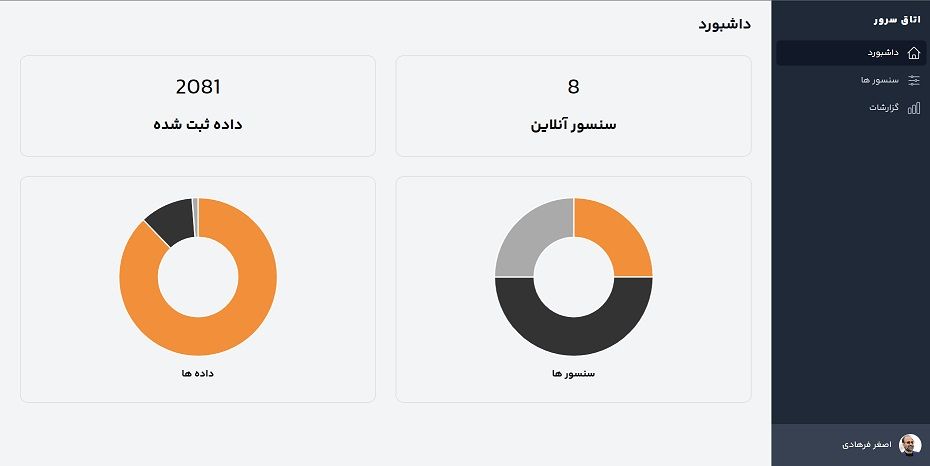
\includegraphics[width=\textwidth]{panel_dashboard}
        \caption{Dashboard tab in the panel}
        \label{panel_dashboard}
    \end{figure}
    \subsection{Sensors}
    The sensors overview page provides a detailed view of the sensors in the server room and as it can be seen in the image \ref{panel_sensors}, user can edit the sensor information or view the sensor data.
    \begin{figure}
        \centering
        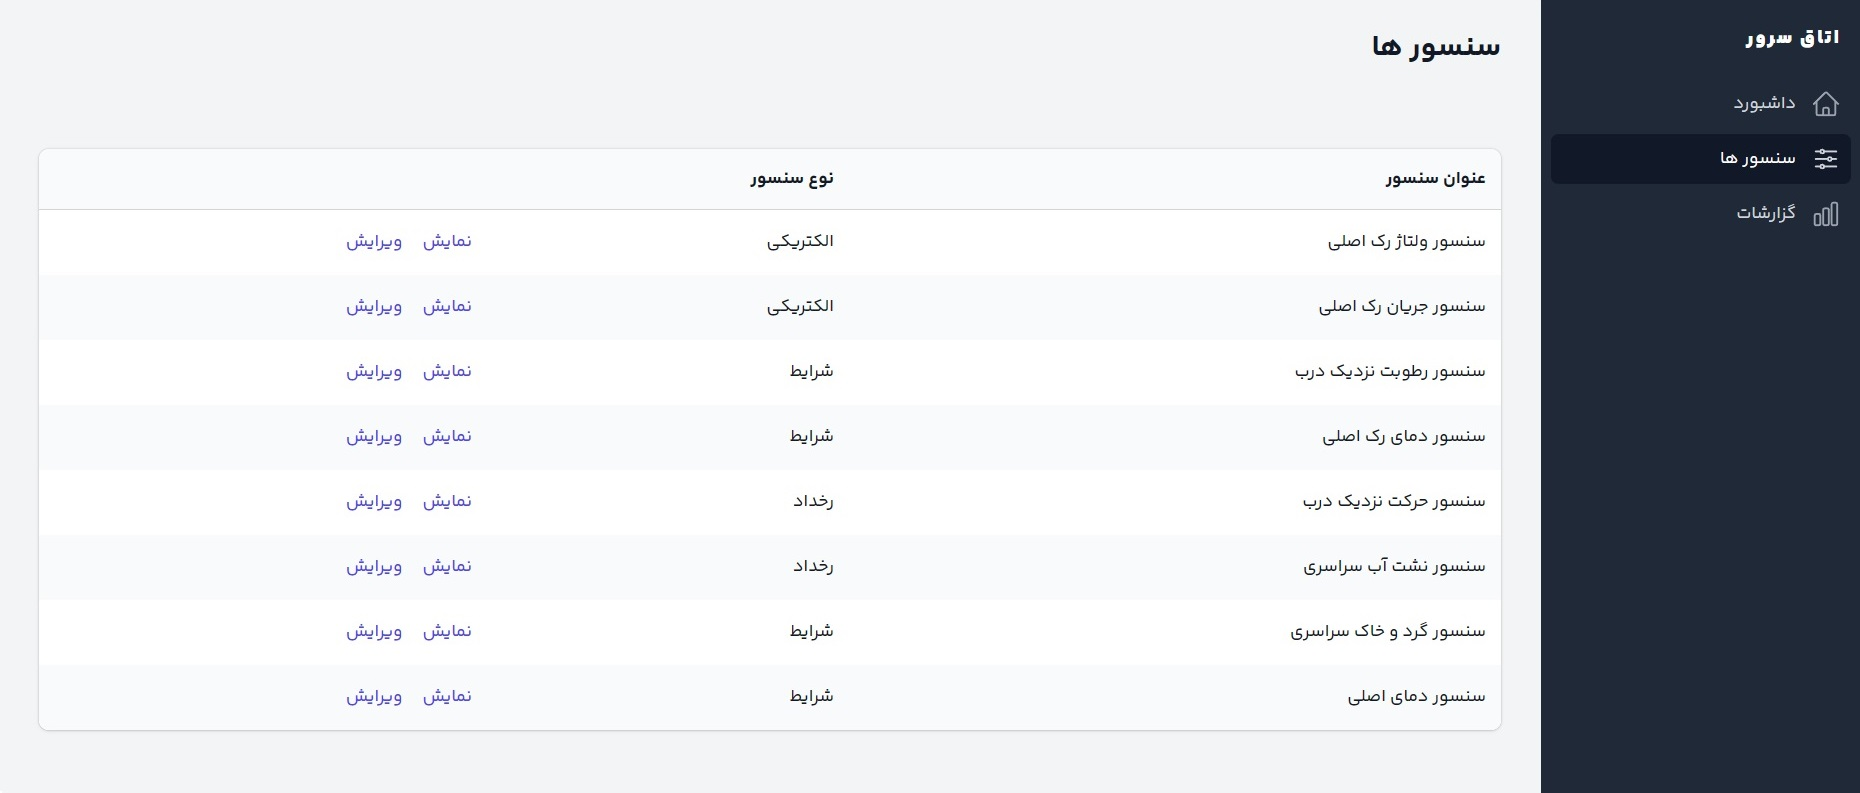
\includegraphics[width=\textwidth]{panel_sensors}
        \caption{Sensors tab in the panel}
        \label{panel_sensors}
    \end{figure}
    \subsubsection{view sensor data}
    The sensor data page provides a detailed view of the sensor data and as it can be seen in the images \ref{panel_dust}, \ref{panel_humidity1} and \ref{panel_temperature1}, user can view the sensor data in a graph.
    \begin{figure}
        \centering
        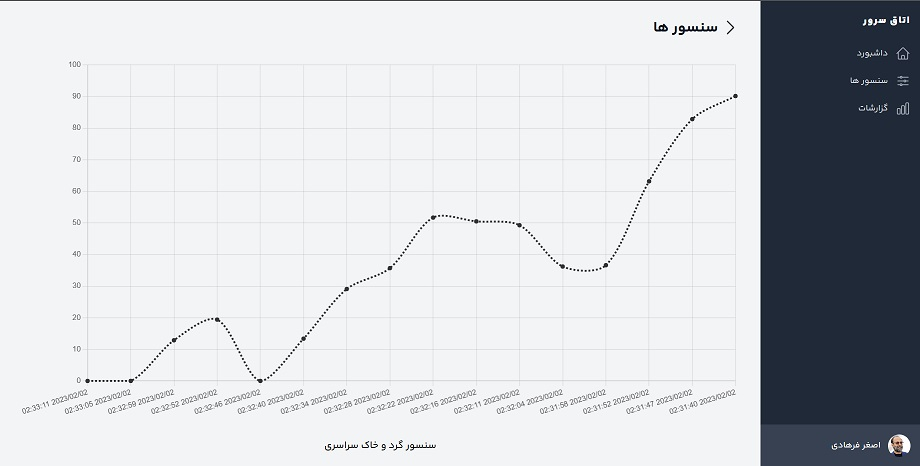
\includegraphics[width=\textwidth]{panel_dust}
        \caption{A dust sensor data in the panel}
        \label{panel_dust}
    \end{figure}
    \begin{figure}
        \centering
        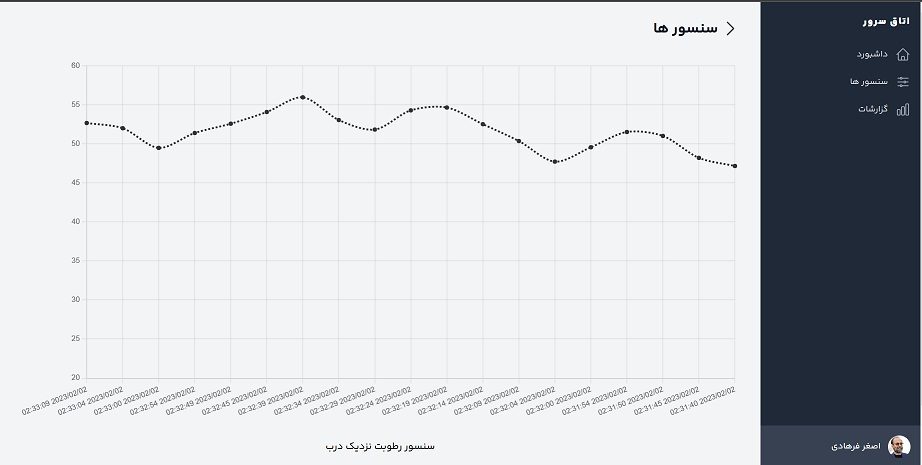
\includegraphics[width=\textwidth]{panel_humidity1}
        \caption{Humidity tab in the panel}
        \label{panel_humidity1}
    \end{figure}
    \begin{figure}
        \centering
        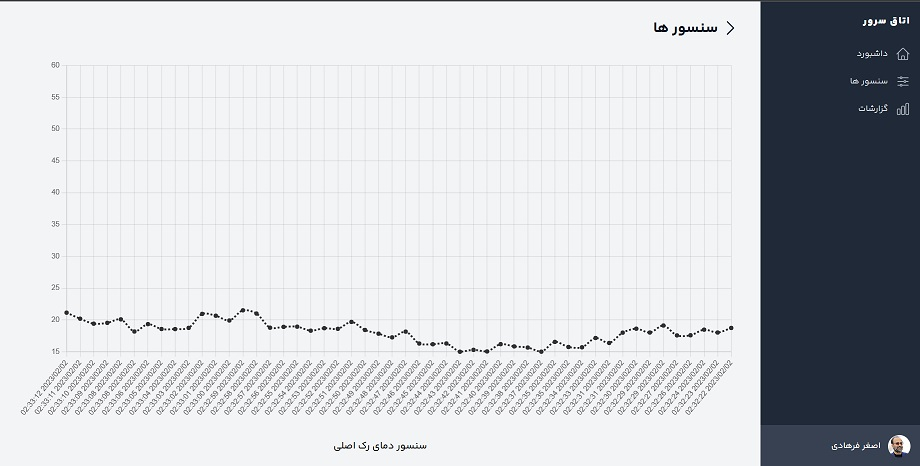
\includegraphics[width=\textwidth]{panel_temperature1}
        \caption{Temperature tab in the panel}
        \label{panel_temperature1}
    \end{figure}
    \subsubsection{sensor settings}
    %In the sensor settings page, user can edit the sensor information and as it can be seen in the image \ref{panel_sensor_settings}, user can edit the sensor name, sensor type, sensor location and sensor threshold.
    In the sensor settings page, user can edit the sensor information and as it can be seen in the image \ref{panel_sensor_settings}, user can edit the sensor's name.
    \begin{figure}
        \centering
        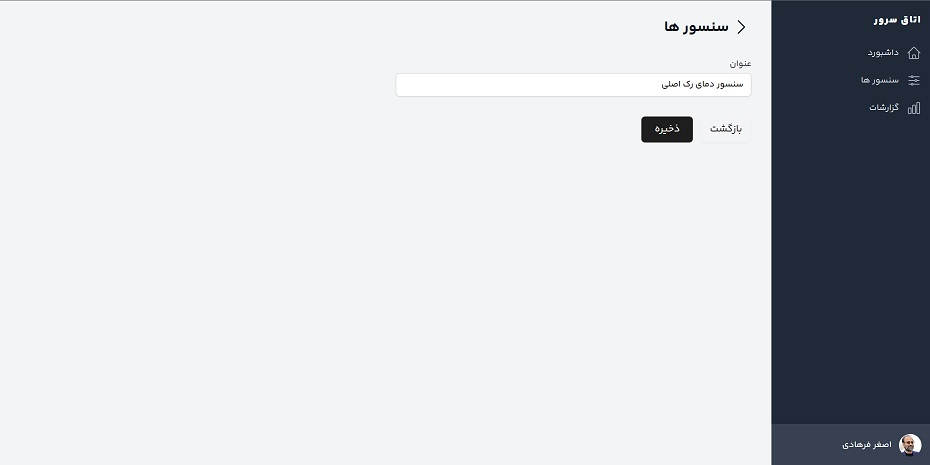
\includegraphics[width=\textwidth]{panel_sensor_settings}
        \caption{Sensor settings tab in the panel}
        \label{panel_sensor_settings}
    \end{figure}
    \subsection{Reports}
    Scatter plots can be an effective way to visualize sensor data because they can help identify relationships or correlations between different sensor readings. In a monitoring system for a server room, multiple sensors are collecting data on various environmental variables, such as temperature, humidity, dust, and so on. By plotting the data collected from different sensors on a scatter plot, it may be possible to identify patterns or correlations between different variables. For example, you might observe that temperature tends to rise as humidity increases, or that there is a relationship between dust levels and humidity changes of the environment. So as it can be seen in figures \ref{panel_sensor_scatter_plot_t_h}, \ref{panel_sensor_scatter_plot_v_i} and \ref{panel_sensor_scatter_plot_h_d}, the relation between temperature and humidity, voltage and current and also humidity and dust has been illustrated in scatter plots. 
    \begin{figure}
        \centering
        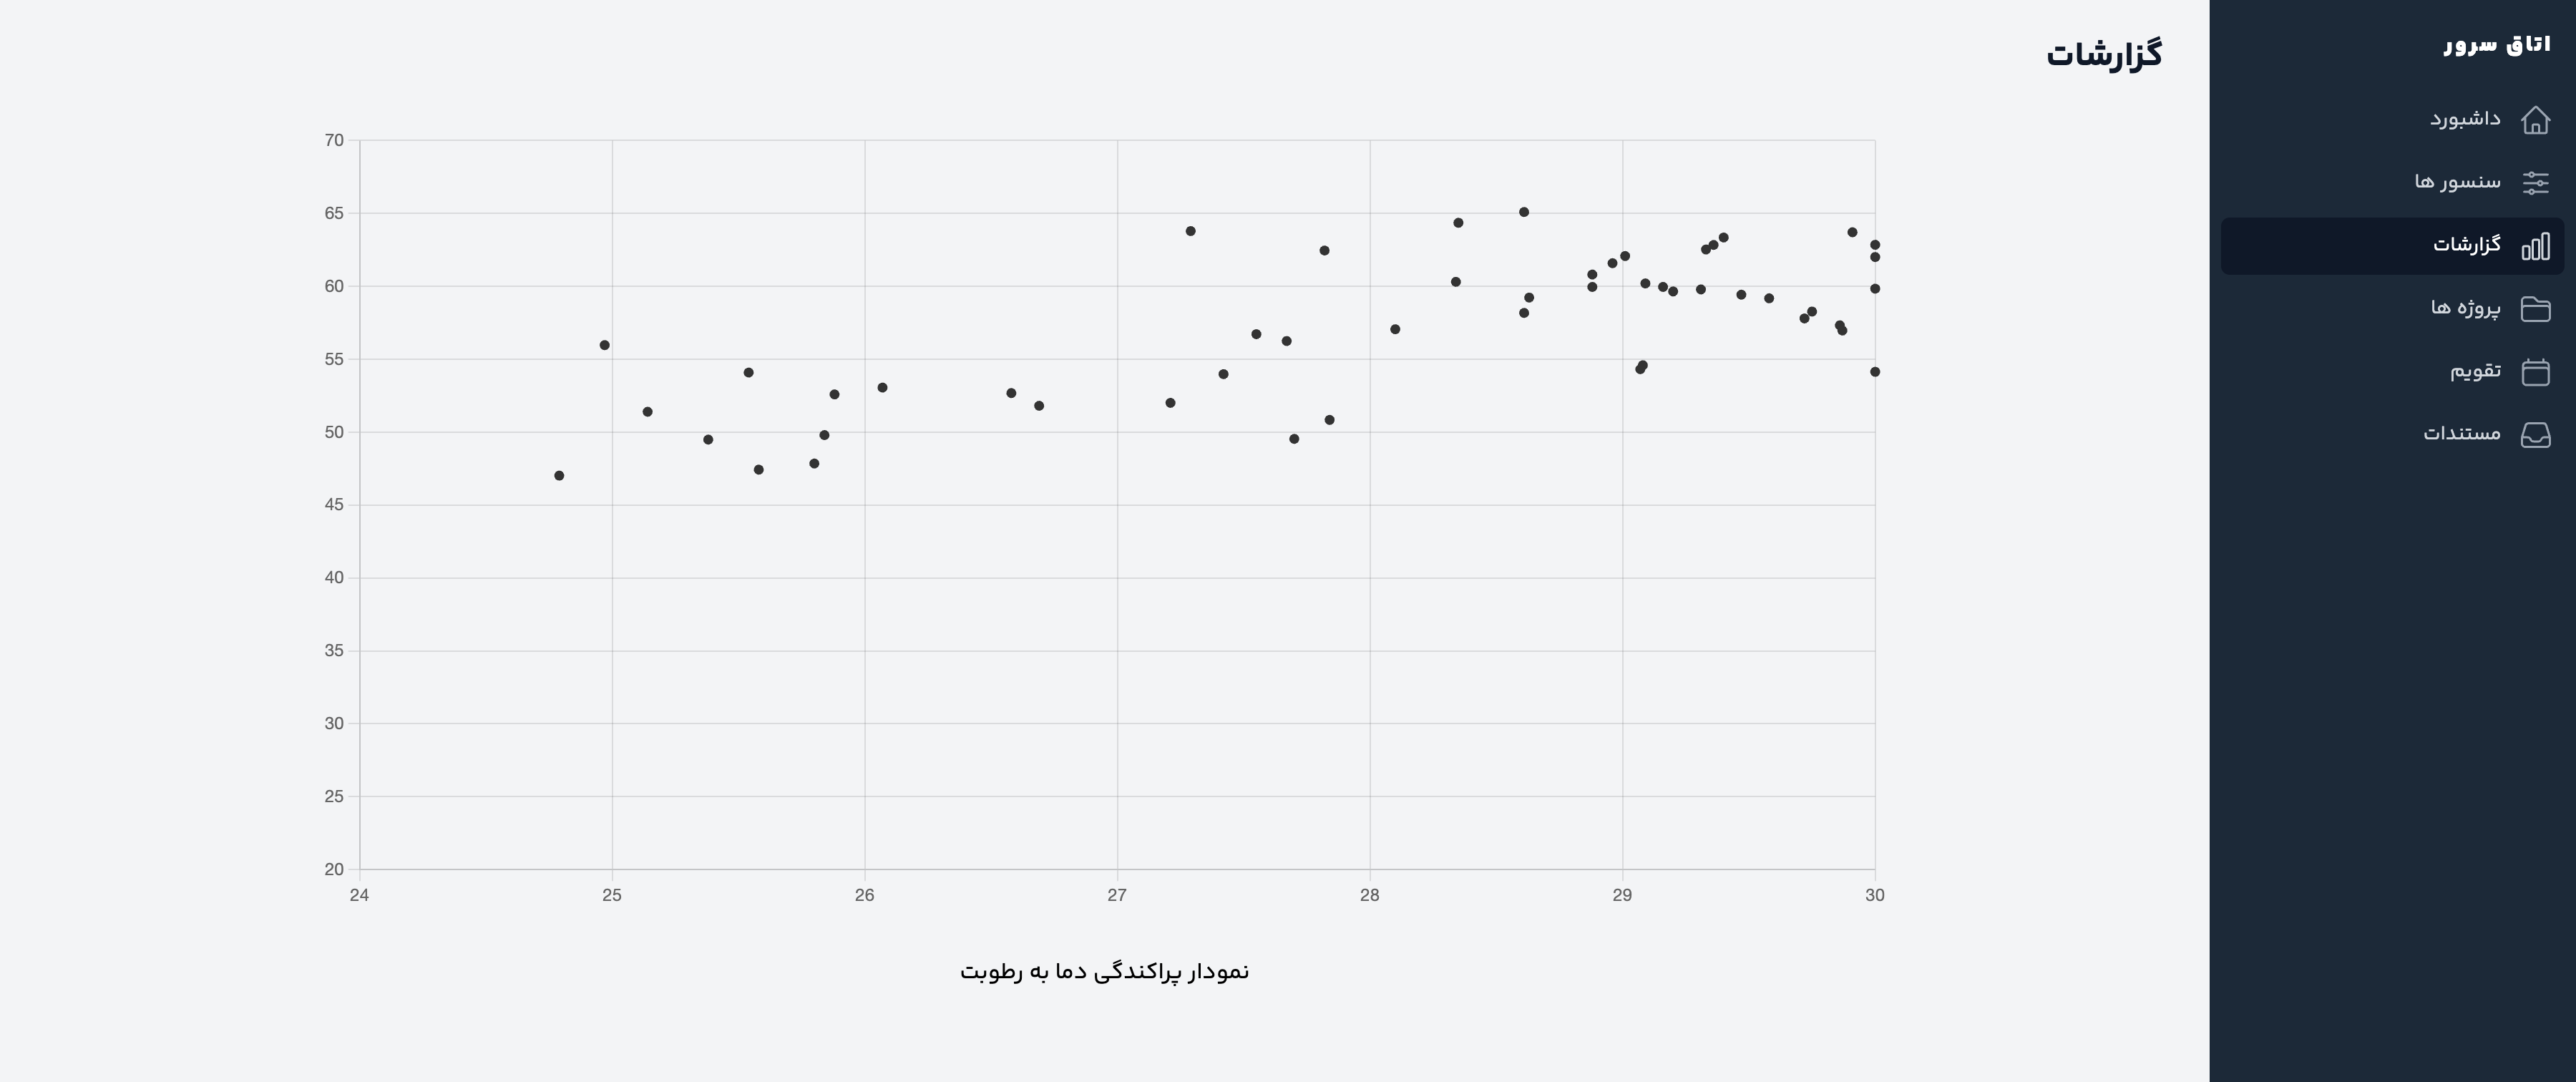
\includegraphics[width=\textwidth]{panel_sensor_scatter_plot_t_h}
        \caption{Relation between recorded data of temperature and humidity sensors}
        \label{panel_sensor_scatter_plot_t_h}
    \end{figure}
    \begin{figure}
        \centering
        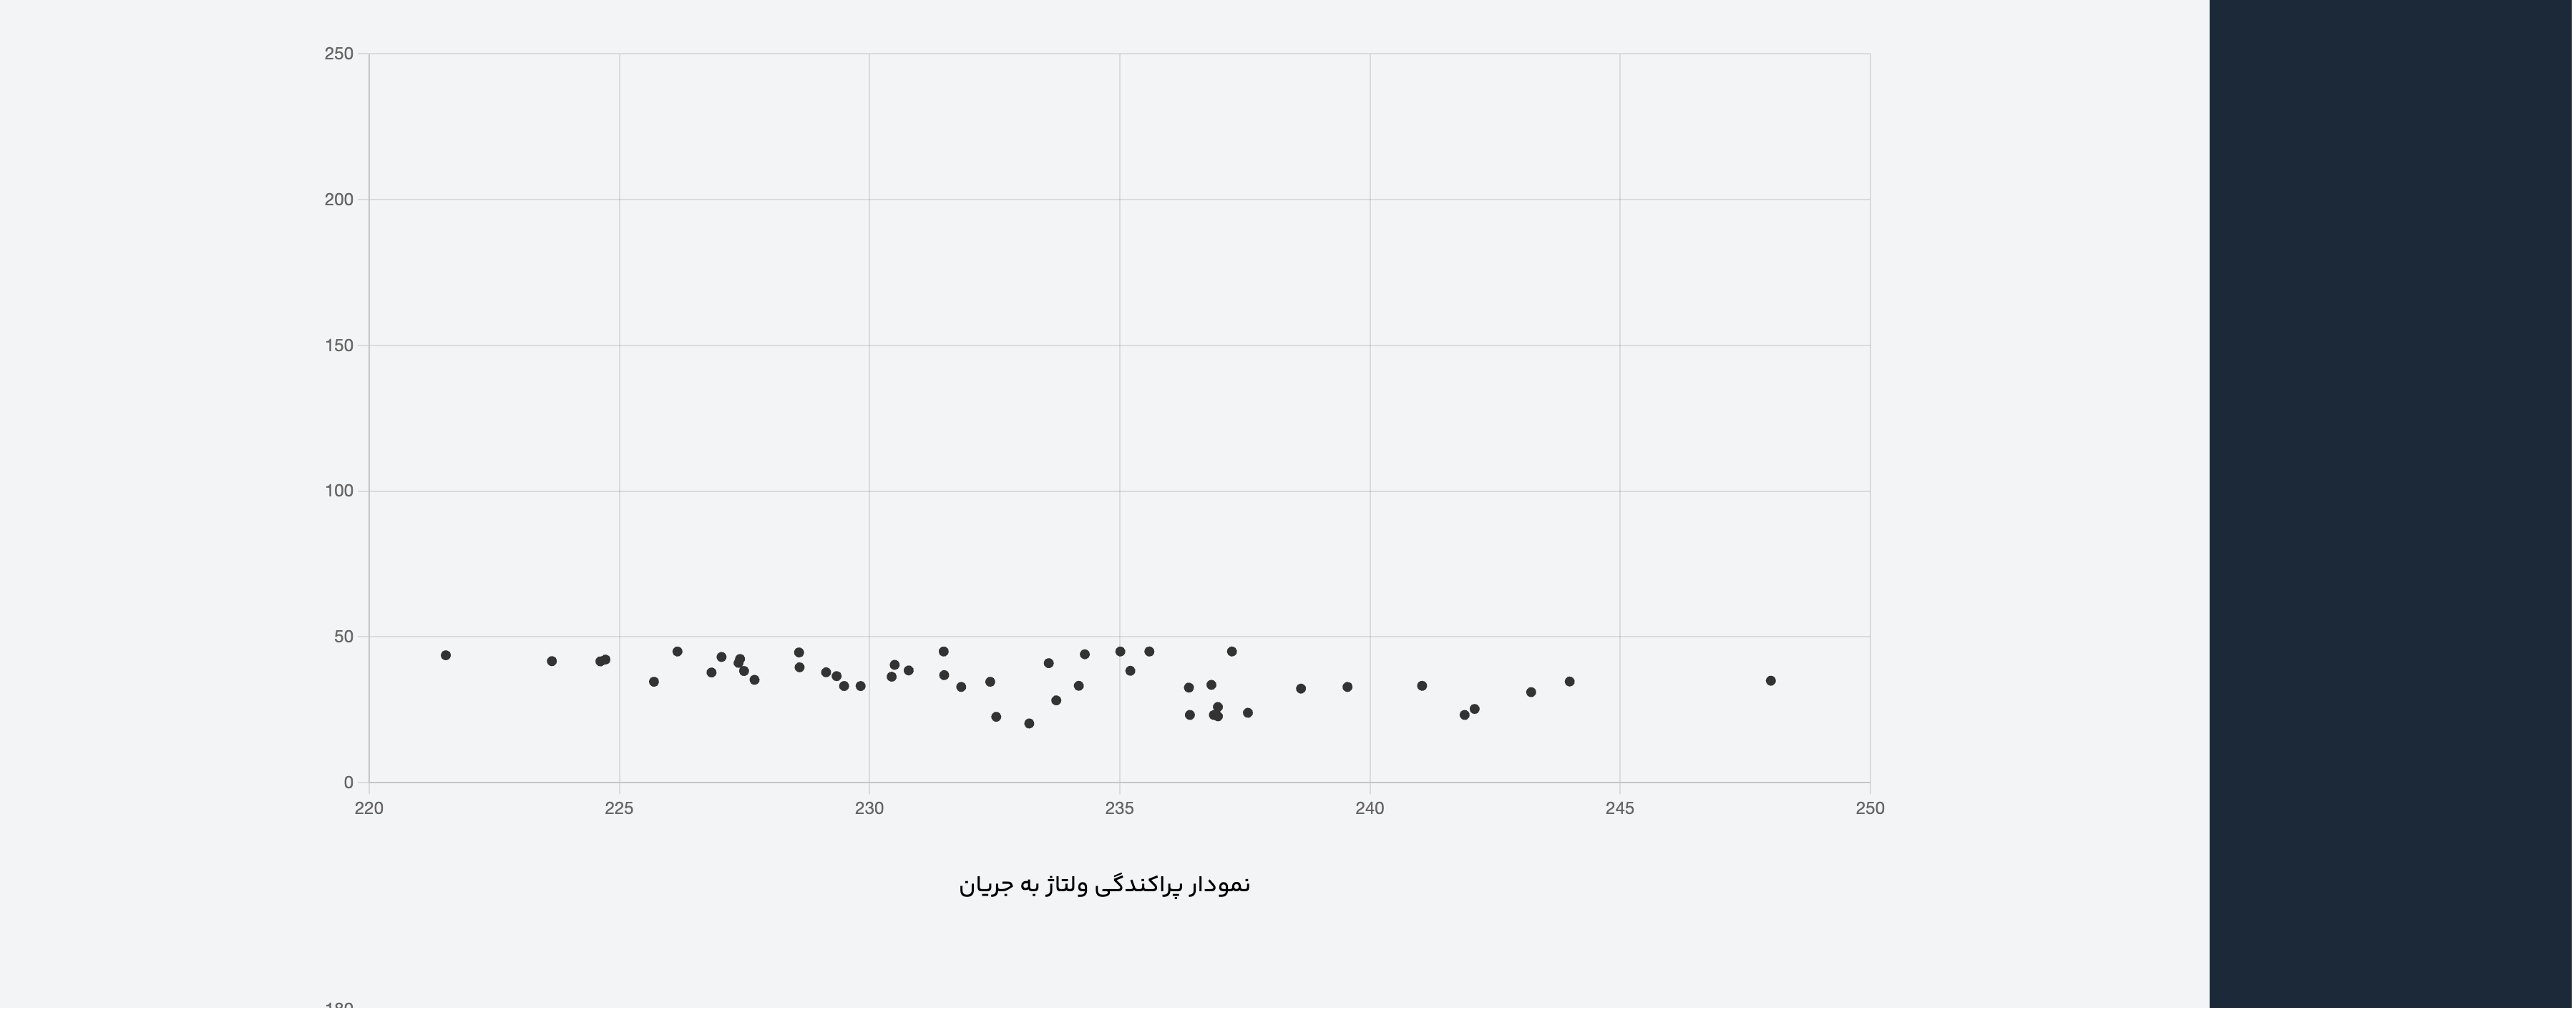
\includegraphics[width=\textwidth]{panel_sensor_scatter_plot_v_i}
        \caption{Relation between recorded data of voltage and current sensors}
        \label{panel_sensor_scatter_plot_v_i}
    \end{figure}
    \begin{figure}
        \centering
        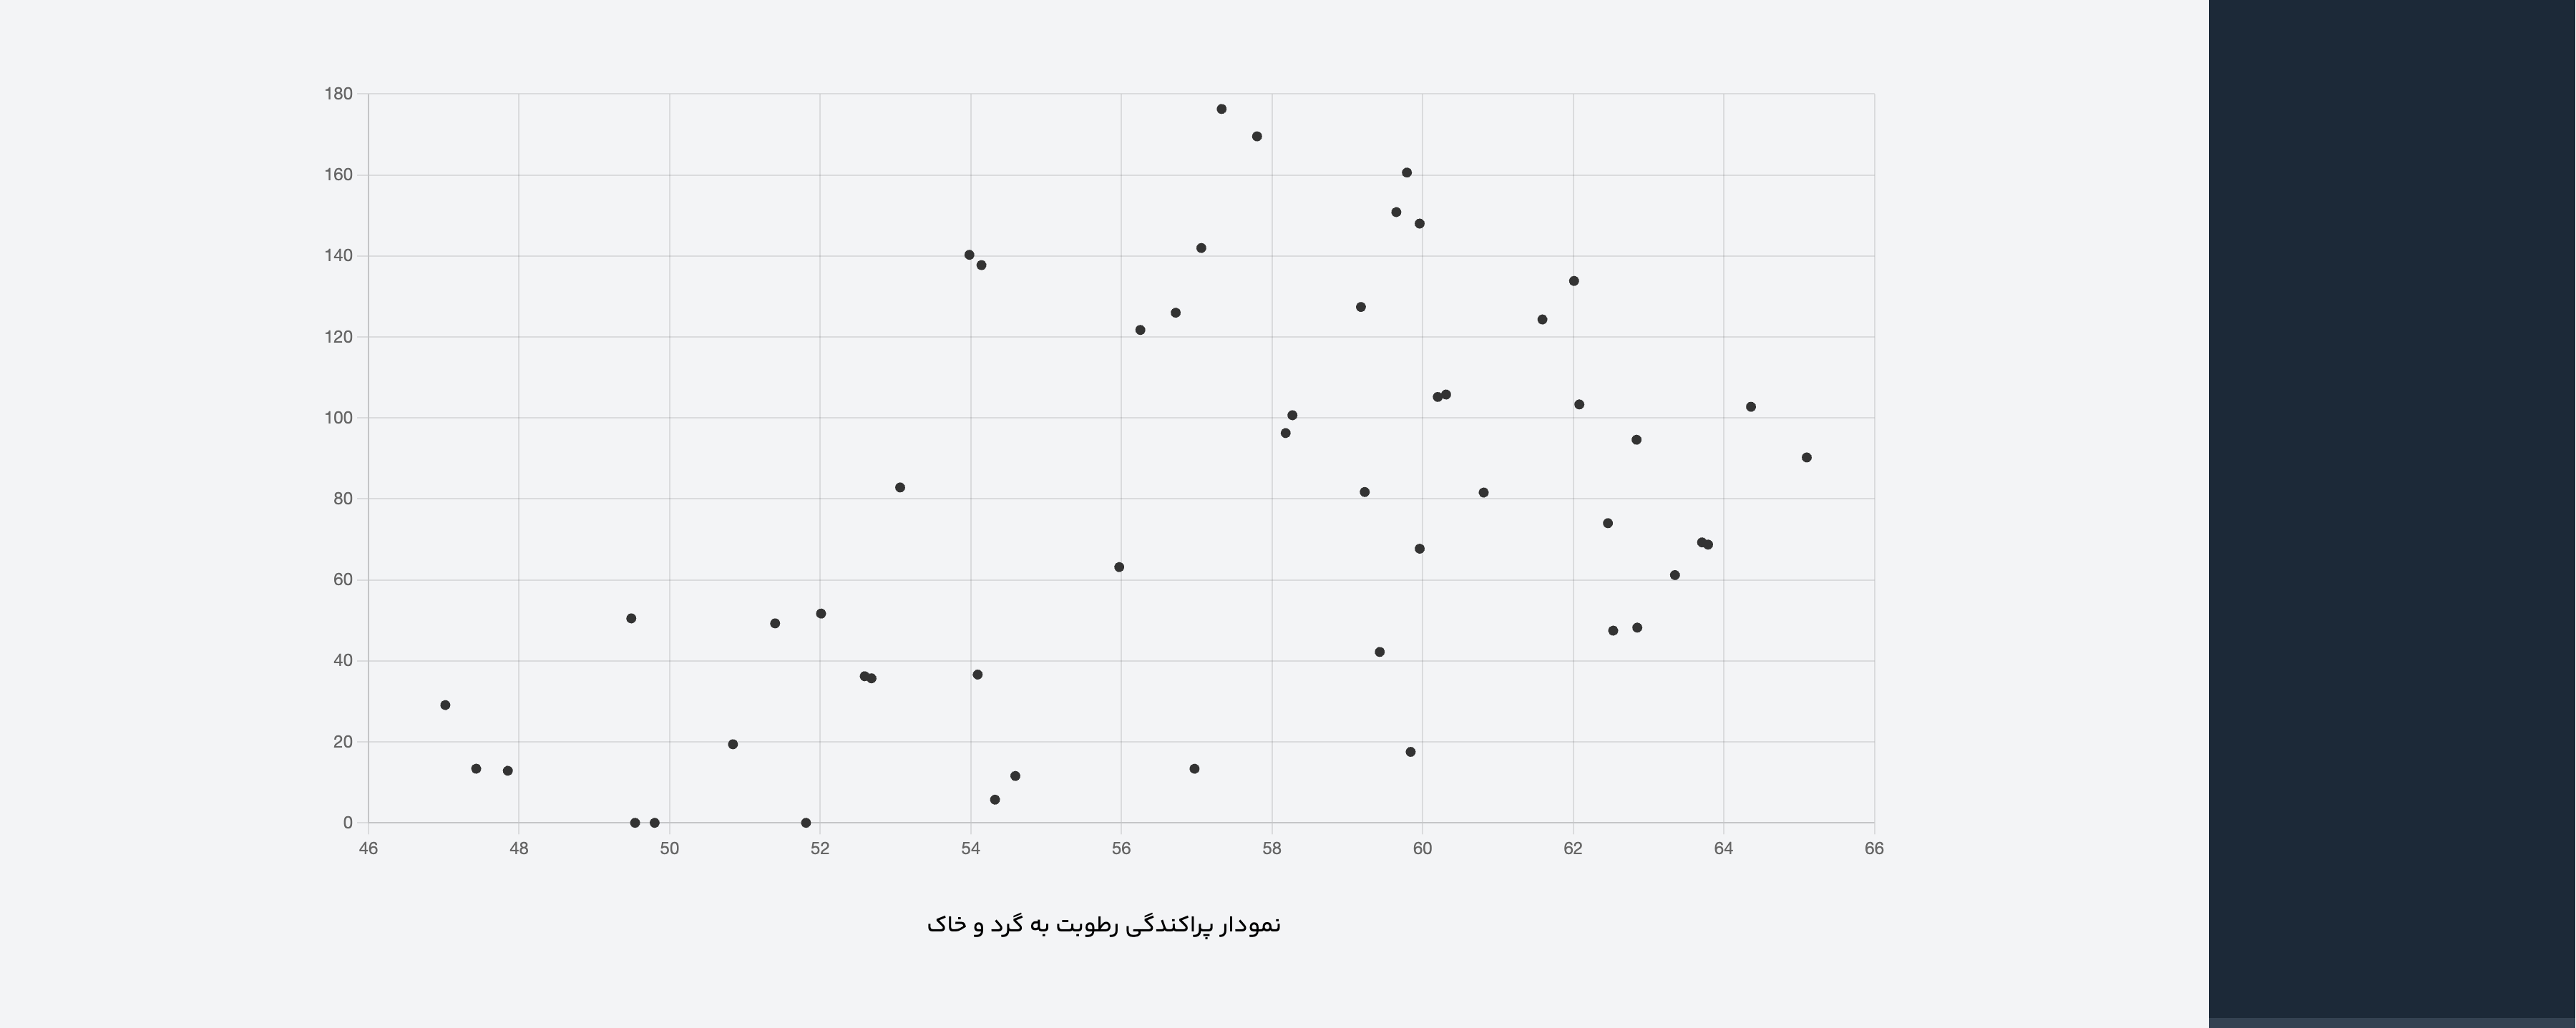
\includegraphics[width=\textwidth]{panel_sensor_scatter_plot_h_d}
        \caption{Relation between recorded data of humidity and dust sensors}
        \label{panel_sensor_scatter_plot_h_d}
    \end{figure}

